\section{Experimentación Final}

Para concluir este trabajo, tomamos todos los algoritmos antes vistos y realizamos una experimentación conjunta entre todos para mostrar como se comparan entre sí.

La primera de las experimentaciones se realizará con grafos completos de 23 vertices con pesos de las aristas elegidas al azar de forma  del 1 al 100. Sobre cada una de estas instancias se correrán todos los algoritmos antes descriptos, se tomarán cual es la mejor solucion encontrada por el mismo y cuanto tarda en encontrarla y en base a los resultados obtenidos se graficarán en una tabla comparativa donde puedan verse los resultados.

De esta experimentación, se obitiene que:

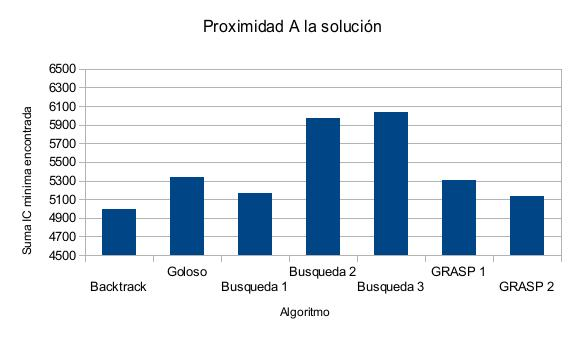
\includegraphics[scale=0.5]{Con/result.jpg}

Nuevamente puede observarse que las mejores heuristicas son las de busqueda local 1 y GRASP 2.

Y los tiempos obtenidos son:

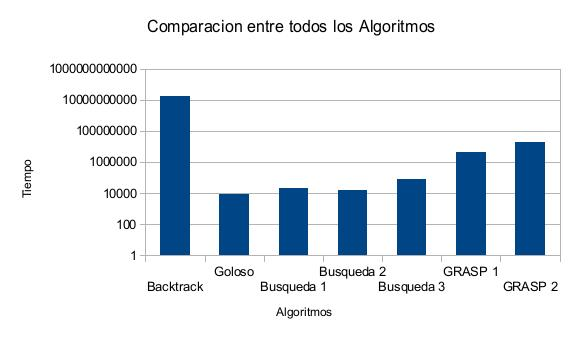
\includegraphics[scale=0.5]{Con/tiempos.jpg}

\section{Conclusión}

Concluimos que dado un problema como $k-PMP$ el cual no conocemos algoritmos polinomiales para resolverlo de forma exacta, podemos utilizar las distintas técnicas algorítmicas para dar una solución en un tiempo razonable con la contrapartida de relajar los requerimientos de la misma. 

Vimos que la técnica de Metaheurística GRASP es una combinación válida entre distintos esquemas de algoritmos y trata de combinarlas para explorar el espacio de soluciones de una manera eficiente. En nuestro caso particular vimos que la implementación de GRASP 2 es la que mejores soluciones encontró. 

Como trabajo adicional habria que hacer pruebas más extensas en distintas familias de grafos conocidas para ver si nuestro algoritmo tiene casos patológicos aun no descubiertos los cuales su solución es tan mala como uno quisiera.